% Compile with pdfLaTeX. Keep screenshots in assets/ next to this
% file.
% Title unnumbered. Main talk: 14 numbered frames. Backup: 4.
\documentclass[aspectratio=169,11pt]{beamer}
\usetheme{Boadilla}
\usecolortheme{default}
\usepackage[T1]{fontenc}
\usepackage{lmodern,amsmath,amssymb,booktabs,graphicx}
\pdfstringdefDisableCommands{\def\translate#1{#1}}
\definecolor{ink}{RGB}{25,48,74}
\definecolor{accent}{RGB}{0,116,125}
\setbeamercolor{structure}{fg=accent}
\setbeamercolor{title}{fg=ink}
\setbeamercolor{frametitle}{fg=ink}
\setbeamertemplate{navigation symbols}{}
\setbeamertemplate{footline}{\hfill\usebeamercolor[fg]{structure}%
\scriptsize\insertframenumber\,/\,14\hspace{5mm}\vspace{3mm}}
\setbeamersize{text margin left=8mm,text margin right=8mm}
\setlength{\tabcolsep}{7pt}
\newcommand{\AD}{\mathrm{AD}}
\newcommand{\AI}{\mathrm{AI}}
\newcommand{\source}[1]{\par\vspace{1mm}{\tiny\color{gray}Source:
Dell'Oro \& Gaetan (2025), #1.}}
\newcommand{\figslot}[4]{%
  \IfFileExists{assets/#1}{\includegraphics[width=#2,height=#3,%
keepaspectratio]{assets/#1}}%
  {\parbox[c][#3][c]{#2}{\centering\color{gray}\textit{#4}%
\par\smallskip\scriptsize Screenshot pending}}}
\title[Space--time extremes]{Flexible space--time models\\for extreme
data}
\subtitle{Lorenzo Dell'Oro and Carlo Gaetan\\\small Spatial Statistics
68 (2025), 100916}
\author{}
\date{}
\begin{document}

% Title page (unnumbered)
\begin{frame}[plain,noframenumbering]
\vspace{6mm}
\begin{flushleft}
{\small\color{accent}PAPER PRESENTATION}
\par\vspace{7mm}
{\fontsize{29}{35}\selectfont\bfseries\color{ink}
Flexible space--time models\\
for extreme data\par}
\vspace{6mm}
{\large Lorenzo Dell'Oro and Carlo Gaetan\par}
\vspace{2mm}
{\small\color{gray}\textit{Spatial Statistics} 68 (2025),
100916\par}
\vspace{4mm}
{\normalsize Presenter \par}
{\normalsize \textbf{Siyan Wang}\par}
{\normalsize University of Connecticut, Department of Statistics\par}
\end{flushleft}
\vspace{5mm}
\note{Introduce this as a statistical methods paper. Rainfall is the
application. The goal is dependence modeling rather than rainfall
forecasting.}
\end{frame}

% Slide 1
\begin{frame}{Research background and motivation}
\begin{itemize}\setlength\itemsep{4mm}
\item Extreme rainfall can occur simultaneously at several nearby
locations.
\item Extreme intensity at one location may weaken rapidly over
subsequent days.
\item Assessing joint risk requires a model for both spatial
co-occurrence and temporal persistence.
\end{itemize}
\medskip
{\color{accent}\textbf{Research question}}\par
\smallskip
{\large How can we model spatially widespread extremes whose
intensity may not persist over time?\par}
\source{Sections 1--2}
\note{Use rainfall to motivate joint modeling before introducing
asymptotic classes. Rapid fading in a particular event does not
itself establish asymptotic independence.}
\end{frame}

% Slide 2
\begin{frame}{Modeling challenges and this paper's approach}
\begin{itemize}\setlength\itemsep{4mm}
\item \textbf{Dependence at high thresholds.}
Block-maxima models target aggregated maxima, while this study
models individual threshold exceedances.
\item \textbf{Different spatial and temporal behavior.}
A direct extension of the spatial scale-mixture model forces the
same asymptotic dependence class in both domains.
\end{itemize}
\medskip
\textbf{This paper:} extend the spatial scale-mixture model to allow
different spatial and temporal extremal dependence classes, with an
estimable mixing parameter.
\medskip

The key distinction is whether dependence persists as the threshold
becomes increasingly extreme.
\source{Sections 1 and 2.2}
\note{The restriction concerns the direct extension described in
Section 2.2, rather than all existing space--time models. Introduce
AD and AI on the following slide to explain persistence in the tail.}
\end{frame}

% Slide 3
\begin{frame}{Upper-tail dependence: AD and AI}
For two observations $X_1=X(s_1,t_1)$ and $X_2=X(s_2,t_2)$,
\[
\chi(u)=\frac{\Pr\{F_{X_1}(X_1)>u,\ F_{X_2}(X_2)>u\}}{1-u},\qquad
\chi=\lim_{u\to{1^{-}}}\chi(u).
\]
{\small $F_{X_1}$ and $F_{X_2}$ are the marginal cumulative
distribution functions (CDFs) of $X_1$ and $X_2$, respectively.}
{\small $u$ is the threshold quantile. $\chi(u)$ is the conditional probability}
\smallskip
\begin{columns}[T]
\column{.48\textwidth}
\textbf{Asymptotic dependence (AD)}
\[\chi>0\]
The conditional exceedance probability retains a positive limit.
\column{.48\textwidth}
\textbf{Asymptotic independence (AI)}
\[\chi=0\]
The conditional exceedance probability tends to zero.
\end{columns}
\medskip
\textbf{Example:} $\chi(0.95)=0.4$ means that, given $X_1$ exceeds its
own 95th percentile, $X_2$ has 40\% chance of also exceeding its own 95th percentile.
\source{Section 2.1, Eq. (1). Numerical example for illustration}
\end{frame}

% Slide 4
\begin{frame}{A shared temporal factor and a space--time process}
\small
\setlength{\abovedisplayskip}{5pt}
\setlength{\belowdisplayskip}{5pt}
\[
\boxed{X(s,t)=R(t)^\delta W(s,t)^{1-\delta}},\quad 0\leq\delta\leq1.
\]
\begin{itemize}\setlength\itemsep{1mm}
\item $R(t)$: a shared random factor across locations at time $t$.
\item $W(s,t)$: spatial patterns that evolve over time.
\item $R$ and $W$ are mutually independent, with standard Pareto
margins: $\Pr\{R(t)>r\}=1/r$ for $r\geq1$, and likewise for $W$.
\end{itemize}
\smallskip
\textbf{Construction according to the desired dependence class}
\par
Generate mutually independent auxiliary processes $R^*$ and $W^*$.
\begin{itemize}\setlength\itemsep{0mm}
\item \textbf{AI:} Gaussian processes with correlations below one
for distinct indices.
\item \textbf{AD:} Student's $t$ processes with finite degrees of
freedom and nondegenerate pairwise dependence.
\end{itemize}
\[
R(t)=\frac{1}{1-F_{R^*}(R^*(t))},\qquad
W(s,t)=\frac{1}{1-F_{W^*}(W^*(s,t))}.
\]
$F_{R^*}$ and $F_{W^*}$ are the auxiliary marginal CDFs.
The transformations give Pareto margins and preserve AI/AD.
\source{Eq. (8) and Section 4.2}
\note{These process families are possible constructions, not
 definitions of AI and AD. The rainfall application uses Gaussian
R*. A t process requires a shared random scale across indices.}
\end{frame}

% Slide 5
\begin{frame}{Dependence regimes and the role of $\delta$}
\small
\begin{center}
\begin{tabular}{lllll}
\toprule
Model & $R$ & $W$ & $\delta<0.5$ & $\delta>0.5$\\
 & & & space / time & space / time\\
\midrule
1 & AI & AD & AD / AD & AD / AI\\
2 & AD & AI & AI / AI & AD / AD\\
3 & AI & AI & AI / AI & AD / AI\\
4 & AD & AD & AD / AD & AD / AD\\
\bottomrule
\end{tabular}
\end{center}
\normalsize
\begin{itemize}\setlength\itemsep{2mm}
\item $\delta<0.5$: $W^{1-\delta}$ has the heavier tail and determines
the class.
\item $\delta>0.5$: $R^\delta$ determines the temporal class. Sharing
$R(t)$ makes spatial pairs AD.
\end{itemize}
\smallskip
\small At $\delta=0.5$: Model 1 has spatial AD and temporal AI.
Models 2 and 3 are AI in both domains. Model 4 is AD in both.
Space--time pairs follow the temporal class in this table.
\source{Table 1 and Appendices A--B}
\note{Model 1 tests temporal AD versus AI while keeping spatial AD.
Model 3 tests spatial AI versus AD while keeping temporal AI. These
are candidate-specific switches.}
\end{frame}

% Slide 6
\begin{frame}{Simulation study: workflow}
\small
\begin{enumerate}\setlength\itemsep{2mm}
\item \textbf{Specify model and truth.} Set
$\theta_D=(\phi,\psi,\delta)$. The $\phi$, $\psi$ are used to define 
the dependence structure in R(t) and W(s,t), respectively. Vary
$\delta\in\{0.1,0.2,\ldots,0.9\}$ and fix the other generating
parameters.
\item \textbf{Generate datasets.} Simulate $R(t)$ and $W(s,t)$, then
construct $X(s,t)=R(t)^\delta W(s,t)^{1-\delta}$. Generate 200
datasets per $\delta$ and model, using the observed station layout and
sample size.
\item \textbf{Compute tail summaries.} Calculate $\hat\chi(u)$ over
spatial distances and temporal lags at $u=0.90,0.95,0.99$.
\item \textbf{Estimate parameters.} Apply the previously trained
neural network to each dataset's summaries to obtain $\hat\theta_D$.
Estimate all dependence parameters jointly.
\item \textbf{Compare with truth.} Assess bias, variability, and
whether $\hat\delta$ lies on the correct side of $0.5$.
\end{enumerate}
\smallskip
\textbf{Result:} regime discrimination generally works in the tested
settings. Weak-component temporal parameters are harder to recover.
\source{Section 4.3, Figs. 3--5}
\note{The network is trained before this study. The study evaluates
the trained estimator on independent simulated datasets. Dependence
classification in Table 1 follows from proofs, not from this
experiment.}
\end{frame}

% Slide 7
\begin{frame}{Simulation study: recovering the dependence regime}
\begin{center}
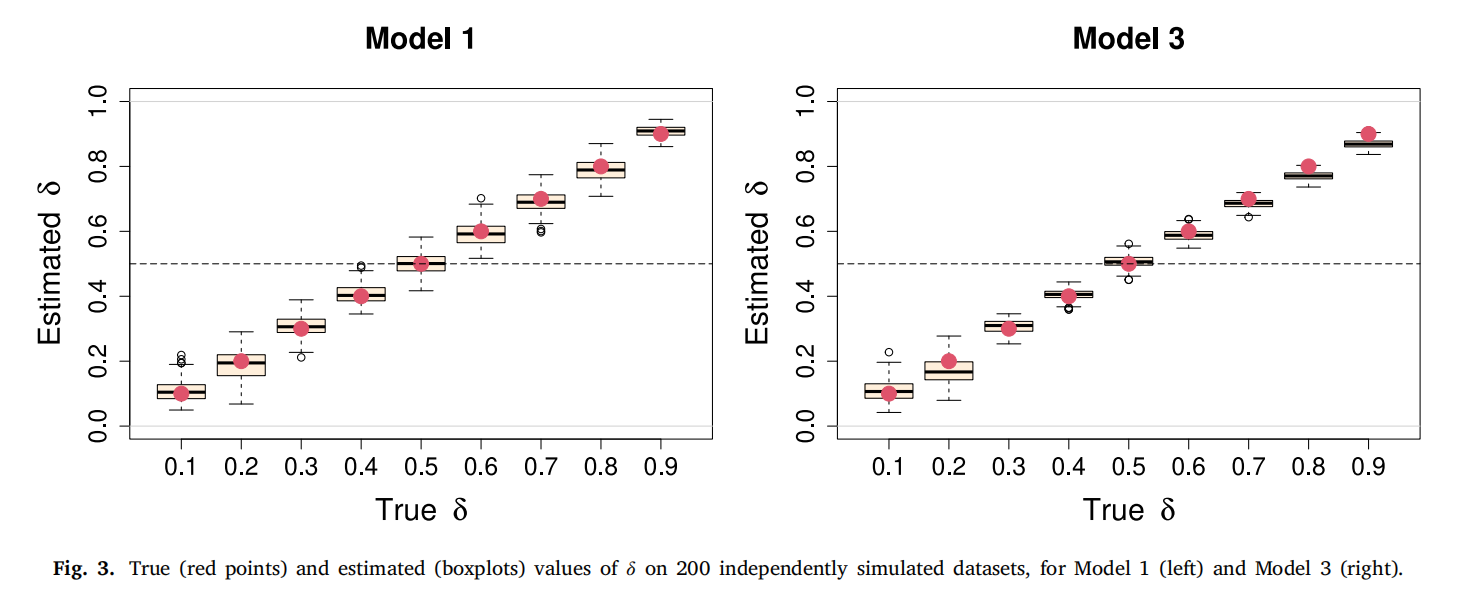
\includegraphics[
  width=\linewidth,
  height=4.25cm,
  keepaspectratio
]{assets/fig3.png}
\end{center}
\vspace{-2mm}
\small
\textbf{Reading the figure:} Red points indicate true $\delta$.
Boxplots show repeated estimates. The dashed line marks $0.5$.
\medskip

\textbf{Finding:} Estimates generally distinguish the two sides of
$0.5$ in the tested settings. 
\source{Section 4.3, Fig. 3}
\note{All dependence parameters are estimated jointly. The nuisance
generating values are fixed in this experiment. This is validation
under an assumed model, not proof of correctness for real rainfall.}
\end{frame}

% Slide 8
\begin{frame}{Rainfall dataset}
\begin{columns}[c,onlytextwidth]
\column{.43\textwidth}
\centering
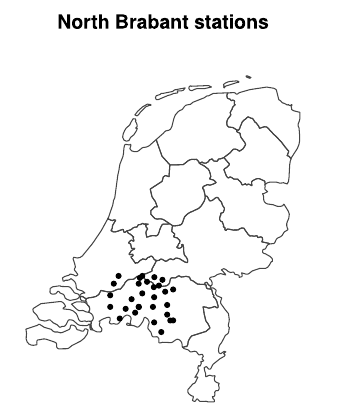
\includegraphics[width=\linewidth,height=5.5cm,keepaspectratio]
{assets/fig1.png}
\column{.53\textwidth}
\textbf{North Brabant, the Netherlands}
\begin{itemize}\setlength\itemsep{2mm}
\item Daily rainfall at 30 stations, 1999--2018.
\item Spring months only: March, April and May.
\item 20 yearly blocks, each with 92 days per station.
\item Temporal dependence within years, assumed independence
between years.
\end{itemize}
\smallskip
\small A small, geographically homogeneous region motivates
stationary dependence modeling over the study domain.
\end{columns}
\source{Section 4.1 and Fig. 1. Data from ECA\&D}
\note{Stations with missing data were excluded. Restricting the
analysis to spring reduces seasonality. Independence between years
is a modeling assumption rather than a property established here.}
\end{frame}

% Slide 9
\begin{frame}{Real-data application: workflow}
\small
\begin{enumerate}\setlength\itemsep{2mm}
\item \textbf{Observe rainfall $Y(s,t)$.}
Use daily spring rainfall from 30 stations over 20 years.
\item \textbf{Explore dependence and select candidate models.}
Compute empirical $\hat\chi(u)$. Select appropriate AD/AI
configurations
 based on empirical evidence.
\item \textbf{Fit the marginal distribution.}
Estimate spatial thresholds $\mu(s)$ and GPD parameters
$\theta_M=(\sigma,\xi)$. The model connects the rainfall scale to
$X$ through $Y(s,t)=Q_{s,t}(G(X(s,t)))$.
\item \textbf{Estimate dependence parameters and uncertainty.}
Input observed tail summaries into each model's trained network to
obtain $\hat\theta_D=(\hat\delta,\hat\phi,\hat\psi_1,\hat\psi_2)$.
Use parametric bootstrap for confidence intervals.
\item \textbf{Interpret and evaluate the fitted models.}
Infer dependence classes from the model and $\hat\delta$. Check tail
diagnostics and compare models using cross-validation.
\end{enumerate}
\smallskip

{\footnotesize\textbf{Note:} The generalized Pareto distribution
(GPD) describes the distribution of exceedance amounts above a high
threshold. $G$ is the marginal CDF of $X$, and $Q_{s,t}$ 
maps uniform quantiles to the threshold-censored rainfall scale.}
\source{Sections 3 and 4.1--4.4}
\note{This is an overview of the analysis, not a strict chronological
claim. Empirical exploration informs candidate selection. The neural
network learns from simulated training datasets. Real observations
supply summaries, rather than a uniquely reconstructed latent X.}
\end{frame}

% Slide 10
\begin{frame}{Exploratory tail dependence}
\begin{center}
\includegraphics[width=.80\linewidth]%
{assets/fig2.png}
\end{center}
\small
\textbf{Empirical tail dependence.}
Curves show $\hat\chi(u)$ from observed joint exceedances at
$u=0.90,0.95,0.99$. Spatial estimates average over time (left),
while temporal estimates average over stations (right).\\[1mm]
Shaded bands show approximate 95\% bootstrap confidence regions.
\\[1mm]
\textbf{Model selection.}
As $u$ increases, spatial estimates remain positive while temporal
estimates approach zero, motivating Models 1 and 3.
\source{Section 4.1, Eq. (11) and Fig. 2}
\note{The curves summarize empirical joint exceedances, rather than
GPD densities or fitted Model 1 and 3 curves. Marginal modeling and
dependence estimation serve different purposes. Finite thresholds
suggest, rather than establish, an asymptotic dependence class.}
\end{frame}

% Slide 11
\begin{frame}{Rainfall results and model comparison}
\begin{columns}[c]
\column{.78\textwidth}
\centering
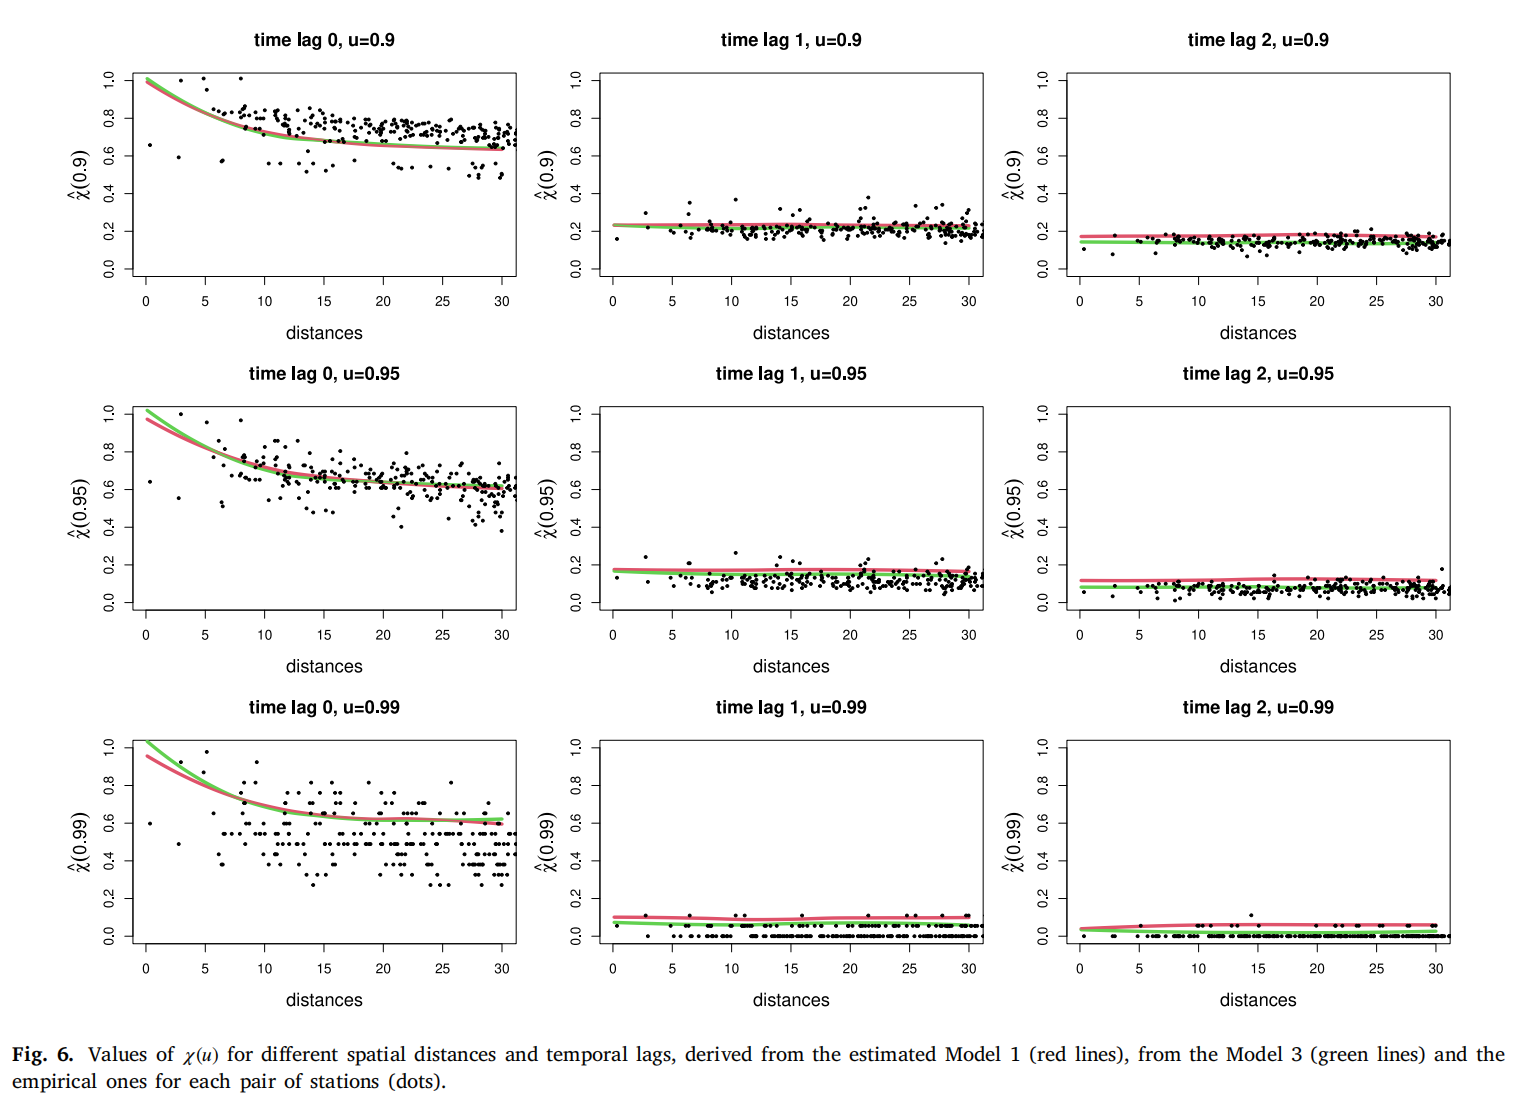
\includegraphics[width=\linewidth,height=7cm,keepaspectratio]
{assets/fig6.png}
\column{.30\textwidth}
\footnotesize
\textbf{Estimates (90\% CI)}\\
Model 1: $\hat\delta=0.577$\\
$(0.519,0.634)$\\[1mm]
Model 3: $\hat\delta=0.631$\\
$(0.585,0.645)$\\[1mm]
Both support spatial AD and temporal / space--time AI.
\medskip

\textbf{Cross-validation}\\
15 years for fitting, 5 for evaluation. Repeat 50 times.\\[1mm]
Tail-summary RMSE:\\
Model 1: $0.066$\\
Model 3: $0.064$\\[1mm]
Slight preference for Model 3.
\end{columns}
\source{Table 2, Fig. 6 and Section 4.4.
Red: Model 1. Green: Model 3. Dots: empirical estimates}
\note{Figure 6 checks finite-threshold fit. Cross-validation compares
held-out tail summaries. The small RMSE difference does not establish
decisive superiority. Neither check directly proves the limiting
class.}
\end{frame}

% Slide 12
\begin{frame}{A simulated rainfall event}
\begin{columns}[c]
\column{.61\textwidth}
\centering
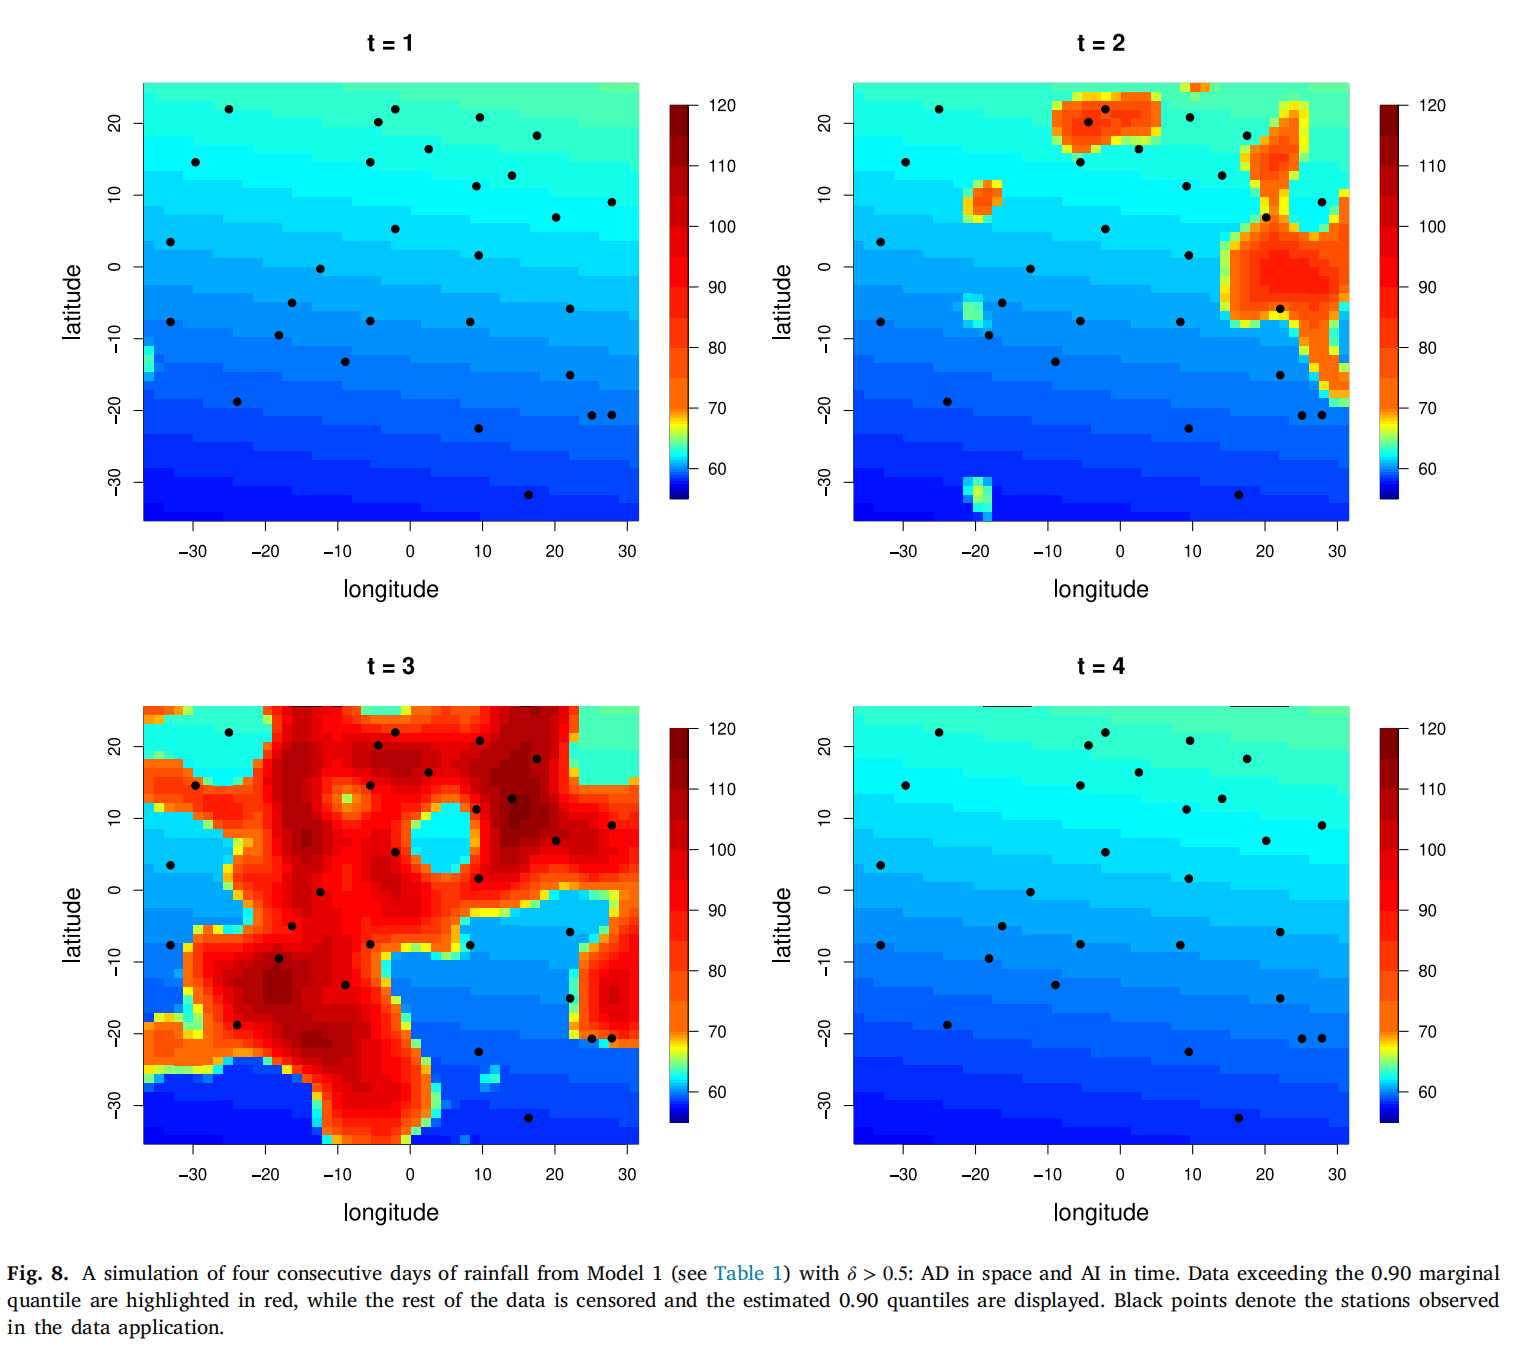
\includegraphics[width=\linewidth,height=7cm,keepaspectratio]
{assets/fig8.png}
\column{.37\textwidth}
\small
Figure 8 shows four consecutive days of rainfall simulated from
fitted Model 1, with $\hat\delta=0.577>0.5$. 

\medskip

Under this model, the estimated parameter implies AD in space and
AI in time.
\medskip

At $t=3$, extreme rainfall affects much of the region, but most
exceedances disappear by $t=4$. This illustrates how extremes can
cluster across locations while fading rapidly over time.
\end{columns}
\source{Fig. 8. Fitted Model 1 simulation, not an observation or
forecast}
\note{The spatially extensive event and rapid fading illustrate the
fitted model's behavior. This single realization does not prove
spatial AD or temporal AI. Blue and green display local thresholds,
not the actual values of simulated rainfall below those thresholds.}
\end{frame}

% Slide 13
\begin{frame}{Contributions and limits of the evidence}
\textbf{Contributions}
\begin{itemize}
\item A stochastic process allowing different extremal classes in
space and time.
\item Simulation-based estimation when likelihood computation is
difficult.
\end{itemize}
\medskip
\textbf{Limits}
\begin{itemize}
\item Finite-threshold fit cannot establish the true limiting class or
latent $W$.
\item Weak mixture components can be difficult to identify.
\item Stationary dependence and the small study region limit
extrapolation.
\end{itemize}
\end{frame}

% Slide 14
\begin{frame}
\begin{center}
{\Huge Thank you!}\\[2mm]
\end{center}
\end{frame}

\appendix
\setbeamertemplate{footline}{\hfill\scriptsize
Backup\hspace{5mm}\vspace{3mm}}

% B1
\begin{frame}{Backup: full dependence table and tail dominance}
\small
\begin{center}
\begin{tabular}{cccccc}
\toprule
Model & $R$ & $W$ & $\delta<0.5$ & $\delta=0.5$ & $\delta>0.5$\\
\midrule
1 & AI & AD & AD / AD / AD & AD / AI / AI & AD / AI / AI\\
2 & AD & AI & AI / AI / AI & AI / AI / AI & AD / AD / AD\\
3 & AI & AI & AI / AI / AI & AI / AI / AI & AD / AI / AI\\
4 & AD & AD & AD / AD / AD & AD / AD / AD & AD / AD / AD\\
\bottomrule
\end{tabular}
\end{center}
Entries: space / time / space--time.
\[
\Pr(R^\delta>x)=x^{-1/\delta},\qquad
\Pr(W^{1-\delta}>x)=x^{-1/(1-\delta)},\quad 0<\delta<1.
\]
The heavier tail determines the class away from $\delta=0.5$.\\
At the boundary, temporal and space--time pairs are AD only if both
components are AD. Spatial pairs inherit the class of $W$.
\source{Table 1 and Appendices A--B}
\end{frame}

% B2
\begin{frame}{Backup: marginal distribution and rainfall
transformation}
\small
For $x\geq1$ and $0<\delta<1$,
\[
G_\delta(x)=
\begin{cases}
1-\dfrac{\delta
x^{-1/\delta}-(1-\delta)x^{-1/(1-\delta)}}{2\delta-1},%
&\delta\ne\frac12,\\[2mm]
1-x^{-2}(2\log x+1),&\delta=\frac12.
\end{cases}
\]
Define $U=G_\delta(X)$ and $Y=Q_{s,t}(U)$. With threshold probability
$p$,
\[
Q_{s,t}(u)=
\begin{cases}
\mu(s,t),&u\leq p,\\
\mu(s,t)+\dfrac{\sigma}{\xi}\left[\left(\dfrac{1-u}{1-p}%
\right)^{-\xi}-1\right],&u>p,\ \xi\ne0,\\
\mu(s,t)-\sigma\log\left(\dfrac{1-u}{1-p}\right),&u>p,\ \xi=0.
\end{cases}
\]
The transformation preserves $\chi(u)$ for $u>p$. Values below the
threshold are censored, so inversion there is not unique.
\source{Eqs. (5), (9), and (10)}
\end{frame}

% B3
\begin{frame}{Backup: simulation and neural estimation details}
\small
\begin{itemize}\setlength\itemsep{1.5mm}
\item Input: three $8\times8$ grids at $u=0.90,0.95,0.99$, treated as
channels.
\item Spatial distances up to 34 km. Temporal lags from 0 to 7 days.
\item Two-dimensional convolution followed by dense layers. Mean
absolute error loss.
\item 30,000 parameter vectors, 20\% validation split, 40 epochs,
batch size 128, RMSprop.
\item Training ranges: $\delta\in(0,1)$, $\phi,\psi_2\in(0,2.5)$,
$\psi_1\in(4,16)$.
\item For each model, 400 parametric bootstrap datasets quantify
parameter variability.
\end{itemize}
\medskip
\[
\rho_{R^*}(k)=e^{-k/\phi},\qquad
\rho_{W^*}(h,k)=\frac{e^{-k/\psi_2}}{1+(\|h\|/\psi_1)^2}.
\]
$R^*$ is Gaussian. $W^*$ is Student's $t$ with $\nu=1$ in Model 1,
Gaussian in Model 3. Pareto marginal transformations preserve their
copulas.
\source{Sections 3 and 4.2}
\end{frame}

% B4
\begin{frame}{Backup: parameter recovery and higher-dimensional
checks}
\begin{columns}[T]
\column{.49\textwidth}
\centering\figslot{fig4.png}{\linewidth}{2.65cm}{Figure 4: recovery
under different mixtures}
\column{.49\textwidth}
\centering\figslot{fig5.png}{\linewidth}{2.65cm}{Figure 5: increasing
independent replications}
\end{columns}
\small
Weak-component temporal parameters are harder to identify. More
independent replications improve recovery in the tested settings.
\medskip
A separate diagnostic checks all four nearest neighbors exceeding
their thresholds, conditional on an extreme at the reference station.
\begin{center}
\begin{tabular}{lcc}
\toprule
Same day ($k=0$) & RMSE at $u=0.90$ & RMSE at $u=0.95$\\
\midrule
Model 1 & 0.116 & 0.138\\
Model 3 & 0.111 & 0.109\\
\bottomrule
\end{tabular}
\end{center}
\source{Figs. 4--5 and Table 3. Other lag settings give similar
performance across models}
\end{frame}
\end{document}








